
\documentclass{beamer}
\usepackage[utf8]{inputenc}
\usepackage{graphicx}
\usepackage{wrapfig}
\usepackage{xcolor}






\usetheme{Madrid}

\AtBeginSection[]{
	\begin{frame}
		\vfill
		\centering
		\begin{beamercolorbox}[sep=8pt,center,shadow=true,rounded=true]{title}
			\usebeamerfont{title}\insertsectionhead\par%
		\end{beamercolorbox}
		\vfill
	\end{frame}
}

\title{Replication Study: Machine Labor (Angrist, 2022)}
\subtitle {Research Module Econometrics}
\author{Cristian Gutierrez, Marcel Wachter}
\centering
\date{January 14, 2023}
\begin{document}
\maketitle

\begin{frame}
\frametitle{Overview} 

\begin{itemize}
    

\item Research Question
\item Motivation
\item Theory
\item Replication Study
\item Conclusion
\end{itemize}
\end{frame}


\begin{frame} {Research Question + Main idea of Angrist (2022)}
\begin{itemize}

\item  Angrist (2022) studies utility of machine learning (ML) algorithms for regression-based causal inference using lasso to select control variables for estimates of college characteristics' wage effect.
\item **Add text here**.
\end{itemize}

\end{frame}






\begin{frame}{Motivation}

\flushleft \textbf{**Add text here**}
\vspace{4mm}
\begin{itemize}
    \item Angrist (2022): Selecting the correct controls from a dictionary allows to make valid inference.
    \item **Add text here**
\end{itemize}

\end{frame}


\begin{frame}{Theory}
\begin{flushleft}
\item Consider a standard linear regression model. 
\end{flushleft}
\[
    y_i=\boldsymbol{\beta_0} +\mathbf{x}_i^\prime \boldsymbol{\beta}+\epsilon_i, \quad i = 1, \ldots, n,
    \tag{1}
\]
\begin{flushleft}
It's estimator looks as follows
\end{flushleft}
\[
\hat{\boldsymbol{\beta}}^{\text{OLS}}=\underset{\boldsymbol{\beta}}{\arg \min}\sum_{i=1}^N (y_i-\beta_0-\sum_{j=1}^p x_{i j}\beta_j)^2
    \tag{2}
\]
\begin{flushleft}
where $\mathbf{x}_i=(x_{i1}, ..., x_{ip})$ and $p$ is the number of regressors.
\end{flushleft}
\end{frame}

\begin{frame}{Theory: The Lasso Estimator}

\begin{flushleft}
Now consider a LASSO estimator as 
\end{flushleft}

	\[
	\hat{\boldsymbol{\beta}}^{\text{LASSO}}=\underset{\boldsymbol{\beta}}{\arg \min}\sum_{i=1}^N (y_i-\beta_0-\sum_{j=1}^p x_{i j}\beta_j)^2
		\tag{3}
	\]
\begin{flushleft}
	subject to 
\end{flushleft}
	\[
    \sum_{j=1}^{p}\left|\beta_{j}\right|\leq t
    \tag{4}
	\]
\begin{flushleft}
	combining (3) and (4) we obtain
\end{flushleft}
	\[
	\hat{\boldsymbol{\beta}}^{\text{LASSO}} &=\underset{\boldsymbol{\beta}}{\arg \min}\left\{\frac{1}{2}\sum_{i=1}^N (y_i-\beta_0-\sum_{j=1}^p x_{i j}\beta_j)^2 +\lambda \left(\sum_{j=1}^p |\beta_j|\right)\right\}
	\tag{5}
	\]
\end{frame}


\begin{frame}{Replication Study}
\begin{itemize}
  
\item **Text** \textbf{**Text**}.
\item **Text**. 
\item **Text** .
\end{itemize}

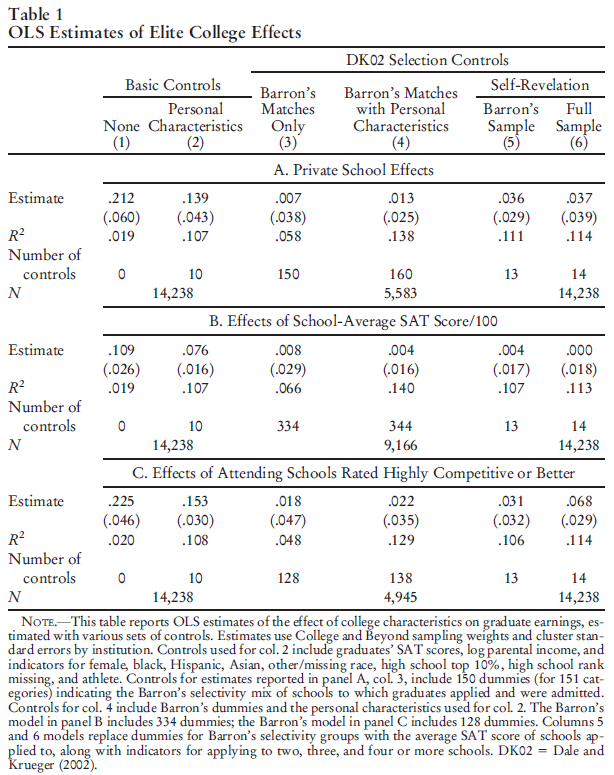
\includegraphics[width=0.4\textwidth]{/Users/marcel/Uni/MSc/3rd/RM_Econometrics/project/rm_econometrics/Presentation/Table 1 Angrist (2022).png}
\end{frame}



\begin{frame} {Conclusions}
\begin{itemize}
\item Data-driven penalties do not improve prediction performance but may ease model interpretation under high sparsity scenarios.
\item Lasso improves the process of feature selection in Labor Economics under approximate sparsity.  
\item ML learning algorithms seem  ill-suited for IV applications in Labor Economics.
\end{itemize}
\end{frame}

\end{document}
